% WACV 2027 paper draft.
\documentclass[10pt,twocolumn,letterpaper]{article}

% \usepackage[review,algorithms]{wacv}
% \usepackage{wacv} % camera-ready
\usepackage[pagenumbers]{wacv} % arXiv

\usepackage{microtype}
\usepackage[dvipsnames]{xcolor}
\usepackage{amsmath,amssymb}
\usepackage{booktabs}
\usepackage{graphicx}
\usepackage{multirow}
\usepackage{pifont}
\usepackage{xspace}

\graphicspath{{figures/}}

\newcommand{\citodo}{\textcolor{BrickRed}{[citation missing]}}
\newcommand{\mat}[1]{\mathbf{#1}}
\newcommand{\vect}[1]{\mathbf{#1}}
\newcommand{\method}[1]{\mbox{\textsc{#1}}}
\newcommand{\dataset}[1]{\mbox{\textsc{#1}}}
\newcommand{\flatsam}{\method{FlatSAM2}\xspace}
\newcommand{\samh}{\mbox{SAM-H}\xspace}
\newcommand{\woftsam}{\mbox{WOFTSAM}\xspace}
\newcommand{\loma}{\mbox{LoMa}\xspace}
\newcommand{\pttst}{PT\textsubscript{TST}\xspace}
\newcommand{\brgap}{\ensuremath{\Delta_{\mathrm{BR}}}}
\newcommand{\bftab}{\fontseries{b}\selectfont}
\newcommand{\frst}[1]{{\bftab#1}}
\newcommand{\scnd}[1]{\underline{#1}}
\newcommand{\cmark}{\ding{51}}
\newcommand{\xmark}{\textcolor{gray}{\ding{55}}}

% Shared paper-figure color key; RGB values match experiments/paper_colors.py.
\definecolor{gtcolor}{RGB}{0,190,90}
\definecolor{flatsamcolor}{RGB}{220,45,120}
\definecolor{woftsamcolor}{RGB}{30,130,230}
\definecolor{sam3color}{RGB}{255,100,0}
\definecolor{maskposecolor}{RGB}{130,60,230}

% Paper-only, supplementary-only, and combined build support.
\newif\ifcombined
\combinedtrue
\newcommand{\xref}[2]{\ifcombined#1\else#2\fi}

% `lineno`'s switch option follows page parity, which puts one two-column
% ruler in the gutter. Select the outer margin from the active column instead.
\makeatletter
\iftoggle{wacvfinal}{}{%
    \renewcommand\makeLineNumber{%
        \if@firstcolumn
            \makeLineNumberLeft
        \else
            \makeLineNumberRight
        \fi
    }%
}
\makeatother

\DeclareMathOperator*{\argmax}{arg\,max}
\DeclareMathOperator*{\argmin}{arg\,min}


% Default: paper only. `make combined` defines \combinedbuild and appends the supplement.
\combinedfalse
\ifdefined\combinedbuild\combinedtrue\fi

\definecolor{wacvblue}{rgb}{0.21,0.49,0.74}
\usepackage[pagebackref,breaklinks,colorlinks,allcolors=wacvblue]{hyperref}

\def\wacvPaperID{*****}
\def\confName{WACV}
\def\confYear{2027}

\title{FlatSAM2: Segmentation-Focused Correspondences\\
for Precise and Robust Planar Tracking}

\author{Jonas Serych\\
Visual Recognition Group, Czech Technical University in Prague\\
{\tt\small serycjon@fel.cvut.cz}
\and
Jiri Matas\\
Visual Recognition Group, Czech Technical University in Prague\\
{\tt\small matas@fel.cvut.cz}
}

\begin{document}
\maketitle

% ===== sec/0_abstract =====
\begin{abstract}
Planar object tracking estimates, for every frame of a video, the homography that maps the planar target from its initial pose to its current one.
Precision and robustness have so far come from different trackers: the best method on the controlled POT-210 benchmark estimates the homography from dense optical flow, computed on the current frame pre-warped by the previous estimate, so that one wrong pose derails every estimate after it; the best method on the in-the-wild PlanarTrack benchmark estimates it from target segmentation masks; neither leads on both.
\flatsam needs no pre-warp: it matches rotation-invariant \loma keypoints between the initial and the current frame and fits the homography by MAGSAC.
Our main contribution is to focus the keypoint proposal with the segmentation the tracker already computes: a planar target covers a median 3.2\% of a PlanarTrack frame, so top-$k$ keypoints land mostly on the background and a small or weakly textured target gets few correspondences; taking in-mask keypoints first and filling the rest from the background lifts the same matcher and estimator from 64.5 to 78.2 p@15 on PlanarTrack, and to 97.3 on POT-210.
A mask-derived pose covers what correspondences cannot, and the same correspondences also name its four cyclically equivalent corners, replacing a separate appearance network with one bounded support score.
The result is a simpler tracker that leads both standard benchmarks at once --- 98.5 p@15 on POT-210 and 88.0 on PlanarTrack --- as well as three further datasets.
\end{abstract}
% ===== sec/1_intro =====
\section{Introduction}
\label{sec:introduction}

Planar object tracking estimates, for every frame of a video, the homography that maps the planar target from its initial pose to its current one.
Unlike generic tracking, a bounding box or a mask is not enough: applications such as augmented reality, visual servoing, and post-production need all eight degrees of freedom of that homography, so that anything registered to the plane stays registered.
Difficult sequences combine blur, occlusion, low resolution, perspective distortion, reflections, and target disappearance, so both short-term precision and long-term recovery matter (\cref{fig:positive-examples}).

\begin{figure*}[t]
    \centering
    % Generate: python experiments/paper_examples.py
    % Copy: cp \
    % /mnt/personal/serycjon/flatsam2/results/experiments/paper_examples/pti_positive.png \
    % paper/figures/pti_positive_examples.png
    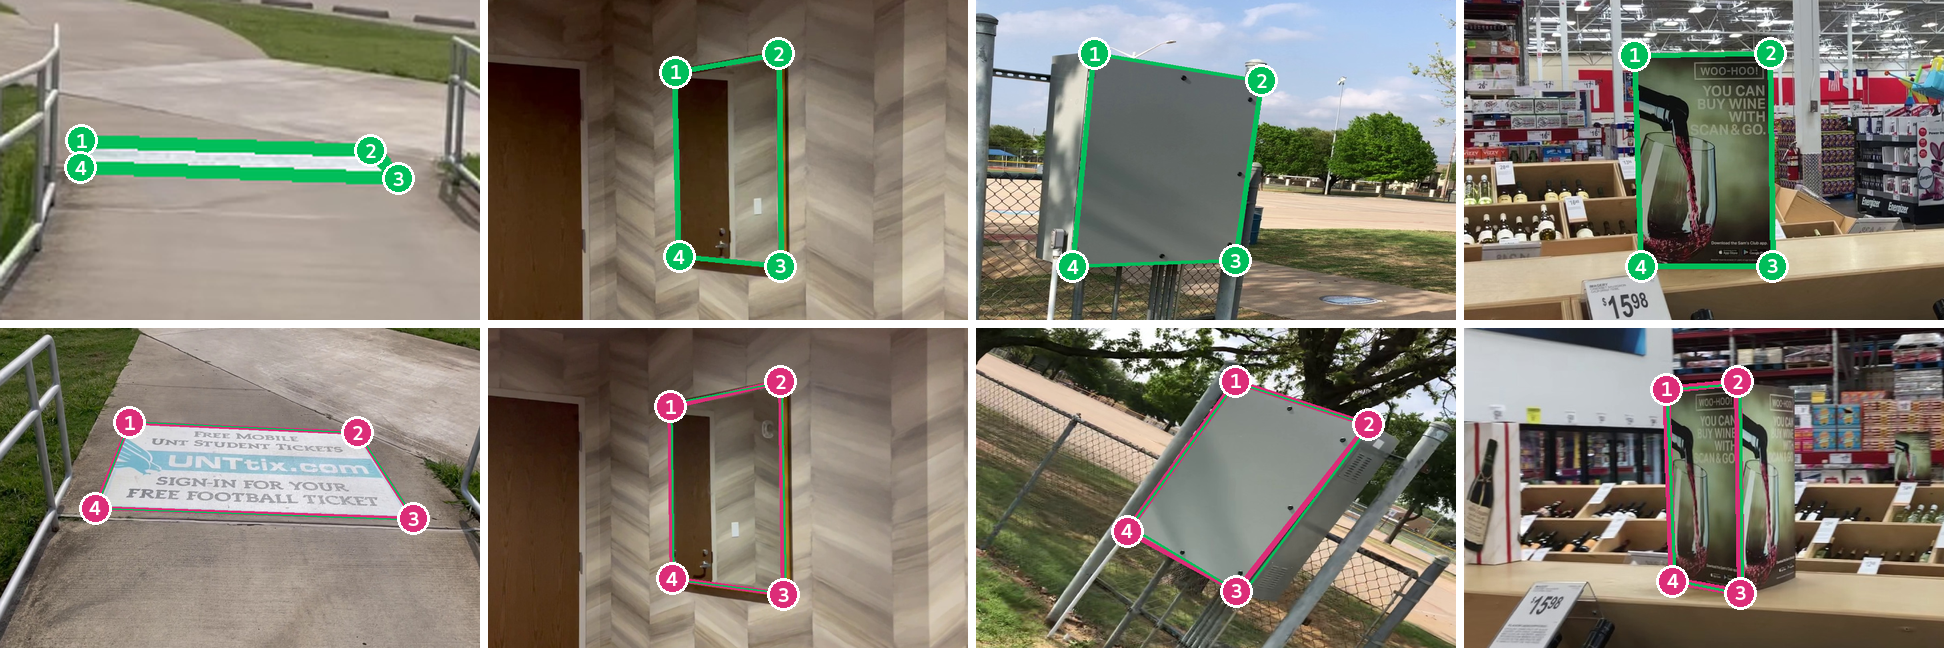
\includegraphics[width=\linewidth]{pti_positive_examples}
    \caption{Positive PlanarTrack~\cite{liu2023planartrack} examples.
    Top: re-annotated initial targets.
    Bottom: later frames with \textcolor{gtcolor}{ground truth} and \textcolor{flatsamcolor}{\flatsam}; numbered markers show corresponding corner identities.
    From left: large scale and perspective change (\texttt{Seq\_00329}, frame 255), reflection (\texttt{Seq\_00341}, frame 40), a textureless surface (\texttt{Seq\_00434}, frame 499), and a planar face on a non-planar package (\texttt{Seq\_00926}, frame 195).}
    \label{fig:positive-examples}
\end{figure*}

Two families of trackers divide this problem, and the division shows in the benchmarks.
Correspondence- and flow-based estimators are geometrically precise while their evidence holds, and they own POT-210, a controlled benchmark of 210 sequences: \woftsam~\cite{serych2026woftsam}, built on dense optical flow, is its strongest published method.
Segmentation-based estimators are robust to blur, texture loss and disappearance, and they own PlanarTrack, an in-the-wild benchmark: \samh~\cite{serych2026woftsam}, which fits a quadrilateral to a tracked mask, is its strongest.
Neither leads on both.
This paper closes that split, with a tracker simpler than \woftsam.

\woftsam inherits its structure from WOFT~\cite{serych2023planar}: the current frame is pre-warped by the last known pose so that the target lands approximately where it was in the initial frame, dense optical flow between the initial frame and the pre-warped frame then measures the small residual motion, and the two are composed into the new pose.
This is very precise while the last pose is approximately right.
When it is not --- after fast motion, an occlusion, or frames without the target --- the pre-warp places different content over the template, the flow between them is meaningless, and every later frame inherits the error.
Recovery has to come from outside the estimator; in \woftsam that is segmentation, and the cascade that arranges it is intricate.

We remove the pre-warp instead of repairing it.
Feature matching originally lost this task because classical descriptors lost correspondences under large viewpoint and appearance change; modern detector--descriptor models do not, and the \loma family~\cite{nordstrom2026loma,nordstrom2026handles} matches across wide baselines and in-plane rotation.
That makes the textbook recipe available again --- match the initial frame to the current frame, fit a homography by RANSAC~\cite{fischler1981random,barath2020magsacpp} --- with no rectification step and nothing carried between frames in this branch.

\noindent\textbf{The textbook recipe alone is not enough.}
Applied to whole frames it reaches 76.1 p@15 on POT-210 and 64.5 on PlanarTrack, far below the flow-based trackers it would replace.
The cause is not the matcher but where its keypoints go.
\loma proposes the top-$k$ peaks of a learned keypoint heatmap over the whole frame, and a planar target is a small part of its frame --- a median 3.2\% of the image area on PlanarTrack.
Although the matcher fires several times more densely on the target, in absolute terms the target collects a median 14.8\% of the correspondences, fewer than 20 of them on 27.8\% of frames; a weakly textured target in front of a textured background gets almost none, and no homography can be fit from what is left.

\noindent\textbf{Segmentation is what makes it work.}
Our main contribution is to spend the keypoint budget where the target is, using the video segmentation model~\cite{ravi2024sam2,carion2025sam} the tracker runs anyway.
Keypoints inside the tracked mask are taken first, up to the full budget, and background keypoints only fill whatever remains.
Nothing is forbidden --- a mask that is too small, late, or wrong still leaves correspondences from the rest of the image to fall back on --- but the target now gets the keypoints it needs.
The same matcher and the same MAGSAC then reach 97.3 p@15 on POT-210 and 78.2 on PlanarTrack, gaining 21.2 and 13.7\,pp over whole-image matching.

\noindent\textbf{Two branches, one mask, simpler interaction.}
Correspondences still run out on textureless surfaces and under heavy blur, so we keep the mask-derived pose of \samh as a second branch and select between the two per frame by keypoint inlier count.
The branches share the segmentation stream and nothing else: neither writes into the other's pose, and the selected output writes into neither.
This replaces \woftsam's three-level cascade, in which the flow estimator is retried on a segmentation-based pre-warp, with one comparison of two complete hypotheses --- and it makes the branches separately measurable, which is how \cref{tab:branch-complementarity} can show that they invert between the two benchmarks.
The same correspondences also resolve the ambiguity specific to the mask branch: a silhouette is unchanged under the four cyclic relabelings of its corners, and where \samh answers this with a DINOv2 appearance model~\cite{oquab2023dinov2} behind six gating parameters, we score each of the four namings by how much of the raw match set its exact four-point homography explains.
One network and six parameters disappear, leaving one distance scale.

Our contributions are:
(i) mask-focused correspondence sampling, which makes a pre-warp-free keypoint branch competitive on small targets in cluttered scenes and is worth 13.7\,pp on PlanarTrack over the same matcher used naively;
(ii) \flatsam, a two-branch tracker that is simpler than the prior cascade --- independent branch states, one selection rule --- and dominates both POT-210 and PlanarTrack with a single model; and
(iii) a simpler and cheaper disambiguation of the mask's cyclic corner symmetry, computed from correspondences the keypoint branch already has, which removes an appearance network and six parameters from the mask branch.
% ===== sec/2_related_work =====
\section{Related Work}
\label{sec:related-work}

\noindent\textbf{Planar tracking and homography estimation.}
Template alignment methods estimate planar motion by directly minimizing photometric or feature residuals, from Lucas--Kanade~\cite{lucas1981iterative,baker2004lucas} and ESM \cite{benhimane2004real,benhimane2007homography} to learned robust representations \cite{chen2019learning}.
Feature pipelines instead detect local evidence, establish correspondences, and fit a homography with RANSAC~\cite{fischler1981random} or robust variants such as MAGSAC++~\cite{barath2020magsacpp}.
Classical SIFT \cite{lowe2004distinctive} and learned descriptors have both been used for this purpose.
The recipe fell behind because classical descriptors lost correspondences under large viewpoint and appearance change; recent detector--descriptor models such as \loma~\cite{nordstrom2026loma,nordstrom2026handles} match across wide baselines and in-plane rotation, which is what allows us to return to it.
Recent trackers also regress control points directly, including HDN \cite{zhan2021homography}, HVC-Net~\cite{zhang2022hvcnet}, and PRTrack \cite{zhang2023multiple}.
WOFT~\cite{serych2023planar} uses dense optical flow after pre-warping the current frame by the previous pose estimate, so that flow is measured between nearly aligned images.
This is what makes flow applicable across a long sequence, and also what ties each estimate to its predecessor: a wrong pre-warp produces flow between different content, with no indication in the flow field that this has happened.
These methods can be highly precise while their evidence remains valid, but recovery after target loss must come from outside the estimator.

\noindent\textbf{Segmentation-guided planar tracking.}
Video object segmentation has gained strong long-term memory and re-detection capabilities, most visibly with SAM~2~\cite{ravi2024sam2} and SAM~3~\cite{carion2025sam}.
A binary mask does not directly provide 8-DoF geometry.
\samh converts a tracked mask into a quadrilateral through Hough line extraction and uses appearance to resolve cyclic corner ambiguity; \woftsam combines this recovery signal with optical-flow homographies \cite{serych2026woftsam}.
Our work retains this useful mask geometry but changes how its corners are identified and how it is paired with a keypoint estimator.
We use one shared segmentation stream but independent homography states, and reuse raw keypoint correspondences as orientation evidence rather than running DINOv2 \cite{oquab2023dinov2} as a second appearance model.

\noindent\textbf{Combining the two.}
\woftsam combines them as a three-level cascade: the flow estimate is retried on a segmentation-based pre-warp before the mask pose is used, so recovery and refinement are entangled and no intermediate estimate is separately meaningful.
Ours is one comparison between two complete hypotheses whose states never touch: a selected keypoint pose cannot alter the mask branch's state, and a selected mask pose cannot alter matching against the initial template.
Besides being simpler, this makes each branch measurable on every frame, which is what a per-frame oracle and the branch analysis of \cref{sec:branch-analysis} require.
% ===== sec/3_method =====
\section{Method}
\label{sec:method}

Given video frames $(I_t)_{t=0}^{T}$ and four initial target corners $X_0=(\vect{x}_1,\ldots,\vect{x}_4)$, the task is to estimate a homography $\mat{H}_t\in\mathbb{R}^{3\times3}$ such that the current corners are $X_t=\mathcal{W}(\mat{H}_t,X_0)$.
The keypoint branch maps the initial frame directly to the current frame; the mask branch uses frame-to-frame composition only when fewer than four corners are visible.
\Cref{fig:overview} summarizes both branches and their final selection.

\begin{figure*}[t]
    \centering
    % Generate: python experiments/paper_overview.py
    % Copy: cp \
    % /mnt/personal/serycjon/flatsam2/results/experiments/paper_overview/overview.pdf \
    % paper/figures/overview.pdf
    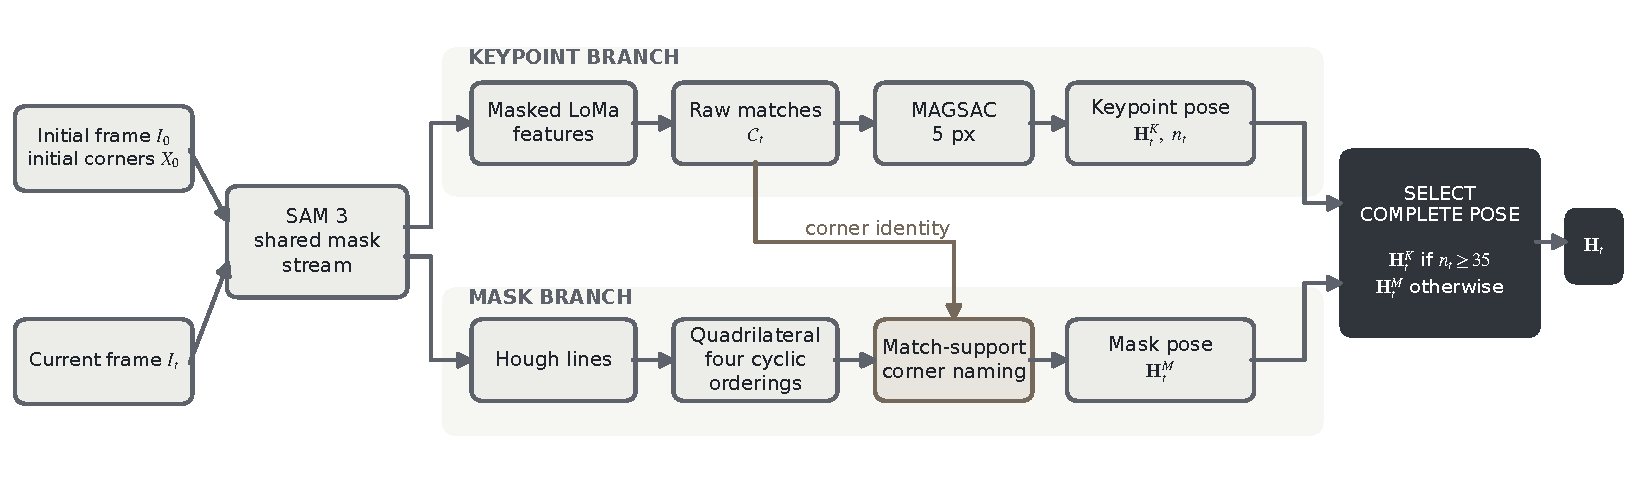
\includegraphics[width=\linewidth]{overview}
    \caption{\flatsam overview.
    SAM3 produces one mask stream consumed by both branches.
    Keypoint correspondences provide a precise homography candidate and, separately, name four cyclic orderings of the mask-derived pose.
    Only final selection is shared; selected outputs do not update either pose state.}
    \label{fig:overview}
\end{figure*}

\subsection{Two Geometric Branches}
\label{sec:two-branches}

\noindent\textbf{Keypoint branch.}
We use the LoMaR~\cite{nordstrom2026handles} variant of \loma~\cite{nordstrom2026loma}, which predicts a dense keypoint score map and local descriptors and is invariant to in-plane rotation.
Matching is always performed between the initial frame and the current frame, never between consecutive frames and never after a pre-warp, so this branch holds no state beyond the cached initial-frame features: $\mat{H}^{K}_t$ does not depend on $\mat{H}^{K}_{t-1}$, and a frame in which matching fails costs exactly that frame.
Matching gives raw correspondences $\mathcal{C}_t=\{(\vect{p}_i,\vect{q}_i)\}_{i=1}^{N_t}$, and USAC-MAGSAC~\cite{barath2020magsacpp} with a 5-pixel threshold estimates $\mat{H}^{K}_t$ and its inlier count $n_t$.
The raw set $\mathcal{C}_t$ is retained before model fitting, for corner naming in \cref{sec:match-naming}.

\noindent\textbf{Mask-focused sampling.}
Which keypoints are matched decides whether the target gets enough correspondences to fit a homography at all: \loma proposes top-scoring peaks over the whole frame, and a small or weakly textured target in front of a textured background gets few of them.
A single non-maximum suppression pass over the score map produces the candidate set, which is then split by the tracked mask, dilated by 10 pixels.
Candidates inside the mask are taken first, in score order, up to the full budget of 4096; background candidates fill only the remainder, $4096-K$ for $K$ selected object keypoints.
The mask is thus a preference, not a restriction.
When it is accurate and the target is small, almost the whole budget lands on the target; when it is late, partial, or wrong, the unspent budget still covers the rest of the image, so target pixels that the mask missed can still be matched and the estimate degrades instead of disappearing.
The initial frame is sampled inside the dilated polygon $X_0$ only: its template features are by construction on the target, and a correspondence is useful only if it starts there.
\Cref{tab:sampling} measures what this preference is worth.

\noindent\textbf{Mask branch.}
SAM3~\cite{carion2025sam}, initialized by the polygon $X_0$, produces binary mask $S_t$.
Following \samh~\cite{serych2026woftsam}, four dominant boundary lines are extracted with a Hough transform~\cite{hough1962method,duda1972use}; valid intersections yield a current quadrilateral and homography $\mat{H}^{M}_t$.
This branch owns its previous homography and partial-visibility state.
It advances on every frame regardless of which branch was selected previously.
It shares the segmentation stream with the keypoint branch, but not its pose or selected output.

With four detected corners, the mask branch estimates the full homography directly.
With two or three corners, it composes its previous homography with a residual similarity transform; with one corner, the residual is translation-only \cite{serych2026woftsam}.

The independence is what keeps one branch's failure local: a confident keypoint fit to the target's mirror image, for instance, cannot drag the mask pose away from the segmented target, and a temporarily malformed mask cannot change the initial-to-current matching problem the keypoint branch solves.
The two complete hypotheses are compared whenever the keypoint homography is available; the mask branch always retains its latest valid pose.

\subsection{Naming Corners by Match Support}
\label{sec:match-naming}

A quadrilateral silhouette is unchanged under four cyclic relabelings of its corners.
Let $X_t^{M,r}$ be mask corners rolled by $r\in\{0,1,2,3\}$ and let $\mat{H}_{t,r}^{M}$ be the exact homography from $X_0$ to $X_t^{M,r}$.
We score each naming against every raw correspondence:
\begin{align}
    d_{i,r} &= \left\lVert
    \mathcal{W}(\mat{H}_{t,r}^{M},\vect{p}_i)-\vect{q}_i
    \right\rVert_2, \\
    U(\mat{H}_{t,r}^{M}) &= \sum_{i=1}^{N_t}
    \max\left(0,1-\frac{d_{i,r}^{2}}{\tau^2}\right),
    \label{eq:match-support}\\
    r^* &= \argmax_r U(\mat{H}_{t,r}^{M}).
\end{align}
The support in \cref{eq:match-support} is measured in effective matches: a perfect correspondence contributes one, support decreases continuously with squared reprojection error, and gross mismatches contribute zero.
Bounded influence is useful on blurred and low-texture frames, where mismatch rates rise.
Unlike a hard inlier count, the score has no decision cliff at $\tau$.
We use $\tau=30$ pixels.

We use pre-MAGSAC correspondences so the naming score sees the complete matcher output and does not inherit the keypoint homography's model-fit filtering.
When fewer than eight matches are available, the mask branch keeps its incumbent naming: eight is twice the four correspondences a homography needs, and below it the four support scores are decided by a handful of matches.
This minimum is fixed for all datasets, and \xref{\cref{sec:supp-naming}}{supplementary Sec.~B} shows the decision is insensitive to it.

The proposed score replaces DINOv2 appearance voting.
It removes a second network and six gating or temporal-consistency parameters, leaving one distance scale $\tau$.
It also runs on every frame with sufficient evidence rather than only after a separate loss detector.

\subsection{Pose Selection}
\label{sec:pose-selection}

The output keeps one branch's complete pose:
\begin{equation}
    \mat{H}_t =
    \begin{cases}
        \mat{H}^{K}_t, & \mat{H}^{K}_t\text{ valid and }n_t\geq T,\\
        \mat{H}^{M}_t, & \text{otherwise},
    \end{cases}
    \qquad T=35.
    \label{eq:selection}
\end{equation}
A keypoint homography counts as valid when at least four correspondences exist, MAGSAC returns a model, and its condition number is finite and below $10^{10}$, which rejects the near-degenerate fits that collapsed or collinear correspondence sets produce.
The selection in \cref{eq:selection} then prefers sufficiently supported correspondences for pixel-level precision, while the segmentation branch is the robust default when support falls.
The branch selected at $t$ is not fed back to either pose state at $t+1$.
$T$ counts inliers rather than thresholding an inlier ratio, because the ratio is not comparable across frames here: background keypoints enter the correspondence set only when the mask leaves budget unspent, so the denominator moves with mask size while the numerator is what the pose is actually fitted from.
\Cref{tab:threshold} shows that $T=35$ lies on a broad plateau.
A branch oracle in \cref{tab:branch-complementarity} quantifies remaining selection headroom.

\subsection{Implementation Details}
\label{sec:implementation}

We use SAM3 in its default streaming configuration and the LoMaR matcher~\cite{nordstrom2026handles}.
Initial and current keypoint sampling masks are dilated by 10 pixels.
Keypoints use $3\times3$ non-maximum suppression and subpixel localization; current and initial budgets are 4096.
Homographies use USAC-MAGSAC, a fixed random seed, and a 5-pixel reprojection threshold.
The mask branch uses the same Hough extraction and partial-visibility handling as \samh~\cite{serych2026woftsam}, restated in \xref{\cref{sec:supp-method}}{supplementary Sec.~A}.
All reported sequences use the same $T=35$, $\tau=30$, and minimum of eight naming matches; the naming parameters were chosen on 50 PlanarTrack \emph{training} sequences, never on a reported test split, and \xref{\cref{sec:supp-naming}}{supplementary Sec.~B} shows both sweeps are flat.
The segmenter is the newest available at the time of writing; \cref{tab:segmenter-control} measures separately how much of our improvement that choice explains.
All runs are deterministic: with fixed seeds, repeated runs on the same hardware are bit-identical.
% ===== sec/4_experiments =====
\section{Experiments}
\label{sec:experiments}

\subsection{Datasets and Metrics}
\label{sec:datasets-metrics}

We evaluate on six planar tracking datasets.
POT-210~\cite{liang2017planar} contains 210 controlled sequences over seven conditions; we use its improved ground truth from~\cite{serych2023planar}.
PlanarTrack~\cite{liu2023planartrack} contains challenging in-the-wild sequences; we use its 300-sequence test split (\pttst) and the precise initial annotations released with \woftsam~\cite{serych2026woftsam}.
POIC~\cite{alismail2016robust} contains 20 sequences dominated by illumination changes.
TMT~\cite{roy2015tracking} contains 92 planar-target sequences recorded during manipulation tasks.
UCSB~\cite{gauglitz2011evaluation} contains 96 controlled sequences spanning six textures and 16 motion or illumination conditions.
MPOT-3K~\cite{zhang2023multiple} is multi-object; each annotated planar instance is evaluated as a separate initialized tracking task, yielding 573 test tasks, so its numbers measure per-plane pose accuracy rather than the benchmark's official multi-object score.

Following prior planar tracking work, alignment error is the RMS corner displacement:
\begin{equation}
    e_{\mathrm{AL}}(\mat{H};\mat{H}^{*},X_0)=
    \sqrt{\frac{1}{4}\sum_{j=1}^{4}
    \left\lVert\mathcal{W}(\mat{H},\vect{x}_j)-
    \mathcal{W}(\mat{H}^{*},\vect{x}_j)\right\rVert_2^2}.
\end{equation}
Precision p@$k$ is the percentage of all annotated frames of a benchmark with $e_{\mathrm{AL}}\leq k$ pixels.

We additionally report best-rotation p@15, which minimizes error over all four cyclic corner orderings.
Its difference from ordinary p@15, $\brgap=\text{BR-p@15}-\text{p@15}$, measures corner-labelling loss while leaving geometric localization unchanged.

\subsection{Main Results}
\label{sec:main-results}

\begin{table*}[t]
    \centering
    \setlength{\tabcolsep}{5pt}
    \begin{tabular}{lccrr|rr}
        \toprule
        & segmentation & geometry & \multicolumn{2}{c|}{POT-210} &
        \multicolumn{2}{c}{\pttst re-annot.}\\
        method & model & branch & p@5 & p@15 & p@5 & p@15\\
        \midrule
        % Published values from the cited papers, as tabulated in the ECCV paper.
        SIFT~\cite{lowe2004distinctive,liang2017planar} & -- & keypoints & 65.8 & 69.6 & -- & --\\
        HDN~\cite{zhan2021homography} & -- & regressed & 70.9 & 92.4 & -- & --\\
        HVC-Net~\cite{zhang2022hvcnet} & -- & regressed & 91.4 & 95.8 & 48.8 & 64.3\\
        WOFT~\cite{serych2023planar} & -- & flow & 90.0 & 95.4 & 48.9 & 65.9\\
        \midrule
        % Result stems: sam_H, sam_H_replay_sam3masks, woftsam_samfallback_nl,
        % woftsam3_guarded (POT) / woftsam_replay_sam3masks (PTi),
        % loma_r_allobj_inflate10, loma_samh_matchnaming.
        \samh~\cite{serych2026woftsam} & SAM2 & Hough & 68.6 & 89.4 & 62.4 & 80.5\\
        \samh, segmenter control & SAM3 & Hough & 70.9 & 90.3 & \scnd{65.0} & \scnd{82.4}\\
        \woftsam~\cite{serych2026woftsam} & SAM2 & flow+Hough & 91.9 & \scnd{97.5} & 57.4 & 77.6\\
        \woftsam, segmenter control & SAM3 & flow+Hough & 92.1 & 97.2 & 58.3 & 79.2\\
        \midrule
        keypoint branch only (ours) & SAM3 & keypoints & \scnd{92.4} & 97.3 & 56.7 & 78.2\\
        \textbf{\flatsam (ours)} & SAM3 & keypoints+Hough & \frst{93.4} &
        \frst{98.5} & \frst{65.6} & \frst{88.0}\\
        \bottomrule
    \end{tabular}
    \caption{Pooled precision on POT-210 and \pttst with re-annotated initial poses.
    Every row below the first block is a complete run scored by the same evaluation code, rather than a number copied from its paper.
    SAM3 controls keep each prior homography estimator fixed, in its original implementation, and replace only the segmenter.}
    \label{tab:main-results}
\end{table*}

\Cref{tab:main-results} compares complete runs on the two primary benchmarks.
\flatsam reaches 98.5 p@15 on POT-210 and 88.0 on \pttst.
The latter is 10.5\,pp above \woftsam and 7.5\,pp above \samh.
On POT, where prior methods already exceed 97 p@15, \flatsam improves by 1.0\,pp over \woftsam.
Its \pttst p@5 is also substantially higher, though p@15 is the primary decision metric because the dataset's annotation uncertainty is significant at five pixels \cite{jiao2025planartrack,serych2026woftsam}.
The keypoint branch alone --- mask-focused \loma correspondences~\cite{nordstrom2026loma,nordstrom2026handles} and MAGSAC, with no pre-warp --- is already within 0.2\,pp of \woftsam on POT-210 and 0.6\,pp above it on \pttst, without the mask branch, the naming rule, or any selection; \cref{sec:sampling-ablation} shows how much of that is the focusing and how much is the matcher.

\begin{table}[t]
    \centering
    \setlength{\tabcolsep}{4pt}
    \begin{tabular}{llrrrr}
        \toprule
        benchmark & estimator & SAM2 & SAM3 & $\Delta$ seg. & \flatsam\\
        \midrule
        % sam_H -> hough_symmetry_only -> loma_samh_matchnaming.
        POT-210 & \samh & 89.4 & 90.3 & +0.9 & 98.5\\
        POT-210 & \woftsam & 97.2 & 97.2 & +0.0 & --\\
        \pttst & \samh & 80.5 & 82.4 & +1.9 & 88.0\\
        \pttst & \woftsam & 78.3 & 79.2 & +0.9 & --\\
        \bottomrule
    \end{tabular}
    \caption{Segmenter control, p@15.
    SAM2 and SAM3 columns keep the homography estimator fixed and differ only in the segmenter; the \woftsam SAM2 entries are re-runs under identical conditions, hence 97.2 / 78.3 rather than the published 97.5 / 77.6.
    \flatsam uses SAM3 and a different combination method.}
    \label{tab:segmenter-control}
\end{table}

\Cref{tab:segmenter-control} separates the segmenter change from the method change.
A newer segmenter helps both prior estimators consistently: \samh gains 1.9\,pp on \pttst and 0.9\,pp on POT, \woftsam 0.9\,pp on \pttst and nothing on POT, which is saturated.
The method contributes several times more.
On top of the same SAM3 masks, our combination adds a further 5.7\,pp on \pttst and 8.2\,pp on POT over \samh, and against whichever prior tracker is strongest with that segmenter --- \samh on \pttst, \woftsam on POT --- \flatsam leads by 5.7 and 1.3\,pp.

\subsection{What Mask-Focused Sampling Buys}
\label{sec:sampling-ablation}

\begin{table}[t]
    \centering
    \setlength{\tabcolsep}{4pt}
    \begin{tabular}{lrrrr}
        \toprule
        & \multicolumn{2}{c}{POT-210} & \multicolumn{2}{c}{\pttst}\\
        keypoint sampling & p@5 & p@15 & p@5 & p@15\\
        \midrule
        % LoMaR__USAC_MAGSAC, loma_r_nogrid_MAGSAC, loma_r_allobj_inflate10,
        % loma_samh_matchnaming.
        whole image, no mask & 65.1 & 76.1 & 43.6 & 64.5\\
        mask first, at most 500 & 90.1 & 95.8 & 54.1 & 75.9\\
        mask first, full budget & 92.4 & 97.3 & 56.7 & 78.2\\
        \midrule
        \textbf{+ mask branch (\flatsam)} & \frst{93.4} & \frst{98.5} &
        \frst{65.6} & \frst{88.0}\\
        \bottomrule
    \end{tabular}
    \caption{Mask-focused sampling.
    Every keypoint row matches the initial frame to the current frame with the same LoMaR model and fits USAC-MAGSAC at a 5-pixel threshold; they differ in which keypoints are matched.
    The first row is the matcher applied off the shelf to whole frames, with its own default keypoint selection and no segmentation.
    The second and third use our sampling with a 4096-keypoint budget and differ in the object cap and a 10-pixel mask dilation.
    The last row adds the mask branch, its naming, and the selection rule, and is the complete tracker.}
    \label{tab:sampling}
\end{table}

\Cref{tab:sampling} isolates the change that makes the pre-warp-free branch work.
The matcher, the robust estimator and the initial-to-current matching problem are the same in all three keypoint rows; what changes is which keypoints are offered to them.
Matching whole frames --- the recipe as it would be applied without a tracker --- loses 21.2\,pp of p@15 on POT-210 and 13.7\,pp on \pttst against the same matcher restricted to the target first.
The intermediate row shows that the effect is graded rather than binary: capping the target at 500 keypoints and spending the remaining 3596 on the background already recovers most of the gap, and lifting the cap recovers the rest.
Mask focusing therefore does not work by removing background correspondences, which are present in all rows, but by ensuring the target has enough keypoints to be matched at all.
This matches the underlying statistics: on \pttst the annotated target occupies a median 3.2\% of the frame and receives a median 14.8\% of whole-image correspondences, with fewer than 20 correspondences on it in 27.8\% of frames --- per unit area the matcher fires three to six times more densely on the target than off it, and is still outnumbered.
The mask branch of \cref{sec:two-branches} then adds 1.2\,pp on POT-210 and 9.9\,pp on \pttst on top of the focused keypoint branch, which is where textureless surfaces and post-occlusion recovery are.

\subsection{Branch Analysis}
\label{sec:branch-analysis}

\begin{table}[t]
    \centering
    \setlength{\tabcolsep}{4pt}
    \begin{tabular}{lrrrr}
        \toprule
        & \multicolumn{2}{c}{POT-210} & \multicolumn{2}{c}{\pttst}\\
        estimate & p@5 & p@15 & p@5 & p@15\\
        \midrule
        % Candidate poses stored by loma_samh_matchnaming (experiments/branch_p_at_k.py).
        keypoint branch & 92.5 & 97.4 & 56.7 & 78.0\\
        mask branch & 70.7 & 90.6 & 65.7 & 84.3\\
        selected output & 93.4 & 98.5 & 65.6 & 88.0\\
        per-frame oracle & \frst{94.5} & \frst{99.0} & \frst{76.2} & \frst{91.2}\\
        \bottomrule
    \end{tabular}
    \caption{Branch complementarity.
    Both branch estimates are scored on every frame, whether or not they were selected.
    The oracle chooses the lower-error branch on each frame using ground truth and is not deployable.
    Our mask branch carries correspondence-support naming, so it is not the same estimator as the \samh rows of \cref{tab:main-results}.}
    \label{tab:branch-complementarity}
\end{table}

\Cref{tab:branch-complementarity} scores the two branch estimates of the deployed tracker separately, and shows why neither prior tracker was strong on both benchmarks.
The branches invert between them: keypoints lead the mask branch by 6.8\,pp on POT-210 and trail it by 6.3\,pp on \pttst.
A tracker built on either alone therefore inherits one benchmark's strength and the other's weakness, which is exactly the \woftsam / \samh split.
Per-frame selection is above the better branch on both, by 1.1 and 3.7\,pp, so the two are complementary rather than redundant.
The one place selection loses is \pttst p@5, where it is 0.1\,pp below the mask branch --- the inlier rule buys a frame's robustness at the occasional cost of a pixel --- and it leads at p@15 regardless.
The remaining oracle headroom is 0.5\,pp on POT-210 and 3.2\,pp on \pttst: POT is nearly saturated, while \pttst is still sensitive to better branch confidence.


\begin{table}[t]
    \centering
    \setlength{\tabcolsep}{3.8pt}
    \begin{tabular}{lrrrrrrrr}
        \toprule
        $T$ & 5 & 15 & 25 & \textbf{35} & 50 & 80 & 150 & 300\\
        \midrule
        % Exact replay from loma_samh_matchnaming stored branch estimates.
        POT-210 & 98.2 & 98.5 & 98.5 & \frst{98.5} & 98.5 & 98.5 & 98.1 & 96.8\\
        \pttst & 83.5 & 87.1 & 87.8 & \frst{88.0} & 88.0 & 87.9 & 87.6 & 87.2\\
        \bottomrule
    \end{tabular}
    \caption{Sensitivity to the keypoint inlier threshold $T$, p@15.
    Bold marks the deployed value.
    Because the selected output never updates either pose state, every threshold can be evaluated exactly from the branch estimates of one run.}
    \label{tab:threshold}
\end{table}

\noindent\textbf{Threshold sensitivity.}
The selection rule's threshold lies on a broad plateau.
\pttst changes by 0.2\,pp over $T\in[25,80]$ and POT is unchanged at the reported precision, so the rule's per-frame discontinuity does not make the tracker sensitive to where the threshold is placed.

\subsection{Cross-Dataset Consistency}
\label{sec:cross-dataset}

\begin{table*}[t]
    \centering
    \setlength{\tabcolsep}{4pt}
    \begin{tabular}{lrrrrrrr|r}
        \toprule
        method & \pttst & POT-210 & POIC & TMT & UCSB & MPOT-3K & worst\\
        \midrule
        % woftsam_samfallback_nl, sam_H, loma_samh_decoupled_rerun,
        % loma_samh_matchnaming.
        \woftsam~\cite{serych2026woftsam} & 77.6 & \scnd{97.5} & \scnd{99.2} & 89.1 &
        \frst{96.6} & \scnd{90.8} & 77.6\\
        \samh~\cite{serych2026woftsam} & 80.5 & 89.4 & 80.8 & 54.3 & 54.3 &
        82.0 & 54.3\\
        \flatsam, DINOv2 naming & \scnd{87.7} & \frst{98.5} & \frst{99.3} &
        \scnd{94.5} & \scnd{92.2} & \frst{92.6} & \scnd{87.7}\\
        \textbf{\flatsam, match naming} & \frst{88.0} & \frst{98.5} & \frst{99.3} &
        \frst{94.7} & \scnd{92.2} & \frst{92.6} & \frst{88.0}\\
        \bottomrule
    \end{tabular}
    \caption{Cross-dataset p@15.
    MPOT-3K p@15 is a per-instance planar tracking diagnostic, not the benchmark's official multi-object metric.
    DINOv2 and match naming variants otherwise share the same tracker; tied first values are both bold.}
    \label{tab:cross-dataset}
\end{table*}

\Cref{tab:cross-dataset} shows the same tracker, unchanged, exceeding both prior trackers on five of six benchmarks.
The weakest-benchmark score, the column that decides whether a tracker is usable everywhere, rises from 77.6 for \woftsam and 54.3 for \samh to 88.0.
The largest difference between the two naming variants is on TMT, where p@15 increases by 0.2\,pp as \brgap falls from 0.36 to 0.03.
The exception is UCSB, where \woftsam reaches 96.6 and both \flatsam variants 92.2; \cref{sec:failure-analysis} examines it.
The same comparison at p@5 and with the corner-naming gap on every benchmark is in \xref{\cref{tab:supp-cross-full} of \cref{sec:supp-results}}{supplementary Sec.~C}.

\begin{table*}[t]
    \centering
    \setlength{\tabcolsep}{4pt}
    \begin{tabular}{lrrrrrrrr}
        \toprule
        method & scale & rotation & perspective & blur & occlusion & OOV & unconstr. & all\\
        \midrule
        % woftsam_samfallback_nl, sam_H, loma_samh_matchnaming.
        \woftsam & 99.3 & 100.0 & 100.0 & 85.0 & 100.0 & 100.0 & 97.9 & 97.5\\
        \samh & 96.0 & 98.6 & 93.9 & 87.9 & 83.7 & 77.0 & 87.3 & 89.4\\
        \textbf{\flatsam} & \frst{100.0} & \frst{100.0} & \frst{100.0} &
        \frst{90.7} & \frst{100.0} & \frst{100.0} & \frst{98.6} &
        \frst{98.5}\\
        \bottomrule
    \end{tabular}
    \caption{POT-210 p@15 by its seven controlled conditions.
    OOV is out-of-view motion.
    Unlike multi-label PlanarTrack factors, each POT sequence isolates one condition.}
    \label{tab:pot-conditions}
\end{table*}

\Cref{tab:pot-conditions} shows that \flatsam retains 100.0 p@15 under scale, rotation, perspective, occlusion, and out-of-view motion.
Blur remains the weakest controlled condition at 90.7 p@15, but improves by 5.7\,pp over \woftsam.

\subsection{Corner Naming Analysis}
\label{sec:naming-analysis}

\begin{table}[t]
    \centering
    \setlength{\tabcolsep}{5pt}
    \begin{tabular}{lrrr}
        \toprule
        naming mechanism & p@15 & BR-p@15 & \brgap\\
        \midrule
        % loma_samh_nonaming, loma_samh_decoupled_rerun, loma_samh_matchnaming.
        none & 85.0 & \frst{89.4} & 4.5\\
        DINOv2 appearance & \scnd{87.7} & \scnd{89.3} & \scnd{1.6}\\
        \textbf{match support} & \frst{88.0} & \frst{89.4} & \frst{1.4}\\
        \bottomrule
    \end{tabular}
    \caption{\pttst naming ablation.
    Lower \brgap is better and isolates corner-labelling errors.}
    \label{tab:naming-ablation}
\end{table}

% Paired sequence bootstrap from the three eval_results.json files: 10,000
% resamples, seed 0, percentile intervals.
\Cref{tab:naming-ablation} shows that match support recovers 3.1\,pp over no naming (95\% CI: 1.9--4.4\,pp) while leaving BR-p@15 unchanged at 89.4.
It therefore changes corner identity without changing localization.
Relative to DINOv2, match support improves p@15 by 0.4\,pp (95\% CI: $-0.4$--1.2\,pp), reduces \brgap by 0.2\,pp, and removes one complete network and six appearance-vote parameters.
POT has zero naming gap and is unchanged at 98.5 p@15 with or without naming, so what the rule buys is \pttst robustness, not precision.
Train-split sensitivity to $\tau$ and the minimum match count appears in \xref{\cref{sec:supp-naming}}{supplementary Sec.~B}.

The rule is active but rarely decisive: over all 147,555 PlanarTrack frames it scores the four namings on 87.2\%, abstains for fewer than eight matches on the remaining 12.8\%, and changes the incumbent naming on 1.75\%.

\subsection{Failure Analysis}
\label{sec:failure-analysis}

UCSB is the one benchmark where \woftsam is stronger, and the deficit is not an arbitration failure.
Over its 6,793 annotated frames \flatsam reaches 92.2 p@15 against \woftsam's 96.6; our keypoint branch reaches 90.7, our mask branch 51.4, and an oracle picking the better of the two per frame would still reach only 93.5.
On 83.4\% of the 530 failed frames neither branch is within 15 pixels, so the loss happens inside the branches, before selection.
Both branches trail \woftsam there, so this is also the one benchmark where dense flow extracts more usable geometry from the target than sparse matching does: UCSB targets are printed photographs and brickwork (median 3.2\% of the frame) viewed under controlled motion, i.e.\ continuous, unoccluded tracking of a repetitively textured plane --- the regime flow was always strongest in, and the one where a robustness mechanism has nothing to recover from.

\begin{figure}[t]
    \centering
    % Generate: python slurm/submit_cmd.py --gpus 0 --no-mail \
    % --job-name ucsb-paper-figure -- \
    % python experiments/ucsb_failures.py --paper
    % Mask source: $OUTPUT_DIRECTORY/ucsb_maskdump/\
    % loma_samh_decoupled_rerun/UCSB/masks/
    % Copy: cp \
    % /mnt/personal/serycjon/flatsam2/results/experiments/ucsb_failures/bricks_perspective__f00044.png \
    % paper/figures/ucsb_target_mismatch.png
    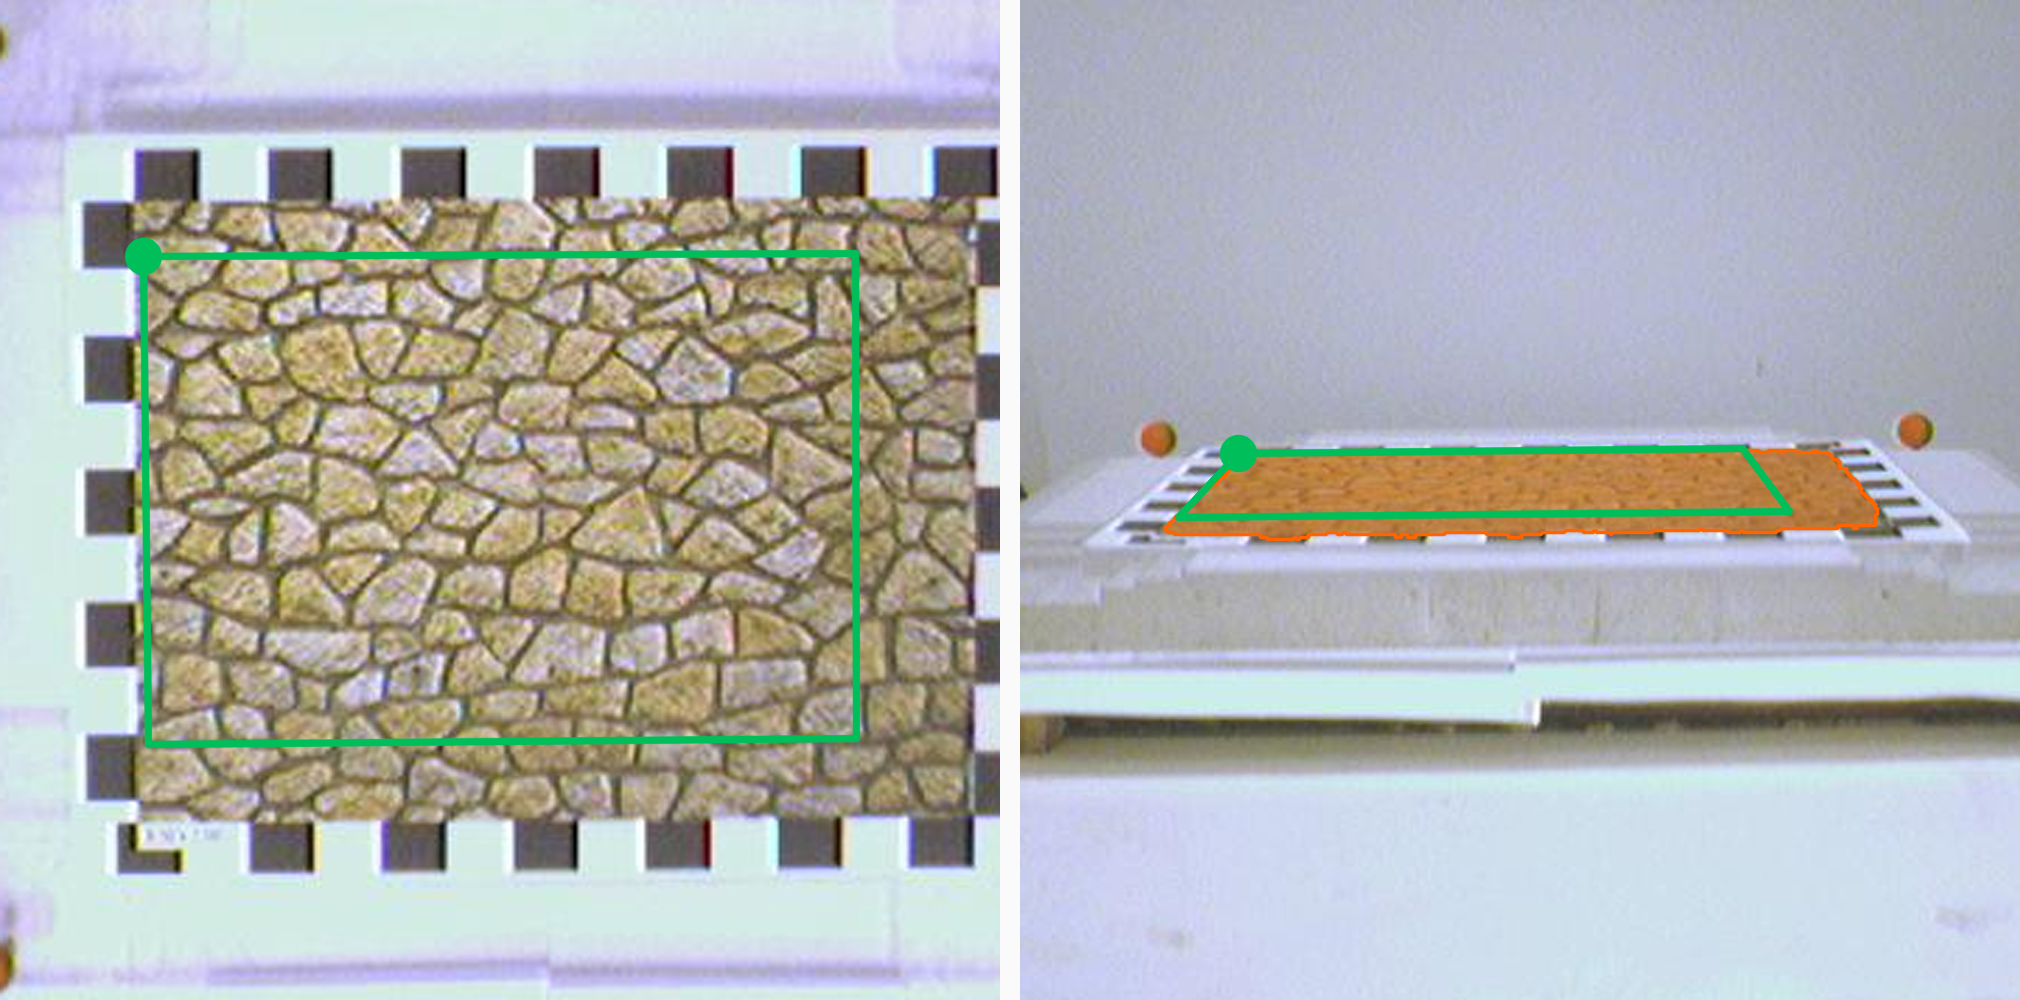
\includegraphics[width=\linewidth]{ucsb_target_mismatch}
    \caption{Representative UCSB target-definition mismatch in
    \texttt{bricks\_perspective}: template (left) and zero-based frame 44
    (right; \texttt{frame00045.jpg}).
    \textcolor{gtcolor}{Ground truth} marks the annotated printed insert in both panels.
    The \textcolor{sam3color}{SAM3 mask}, shown only in the current frame, extends onto the surrounding laminated carrier.}
    \label{fig:ucsb-mismatch}
\end{figure}

Failing mask-based poses share systematically enlarged quadrilaterals, with median linear scale $1.18\times$ relative to ground truth.
In some sequences, segmentation extends beyond the annotated print onto the laminated carrier, as in \cref{fig:ucsb-mismatch}.
In others the mask aligns with the annotated region but quadrilateral fitting is inaccurate, so segmentation scope explains only part of the deficit.
This is not primarily an arbitration failure: both effects occur before branch selection.

\begin{figure}[t]
    \centering
    % Generate: python slurm/submit_cmd.py --gpus 0 --no-mail \
    % --job-name maskpose-strip -- \
    % python experiments/mask_pose_failure.py --panels V22_5:171 V29_3:251 \
    % --results-dir $OUTPUT_DIRECTORY/maskpose_maskdump \
    % --masks-dir $OUTPUT_DIRECTORY/maskpose_maskdump/\
    % loma_samh_matchnaming/POT-210/masks
    % Masks and poses: $OUTPUT_DIRECTORY/maskpose_maskdump/\
    % loma_samh_matchnaming/POT-210/ (--save-masks re-run of the reported config)
    % Copy: cp \
    % /mnt/personal/serycjon/flatsam2/results/maskpose_maskdump/experiments/\
    % mask_pose_failure/V22_5_f00171__V29_3_f00251.png \
    % paper/figures/mask_pose_failure.png
    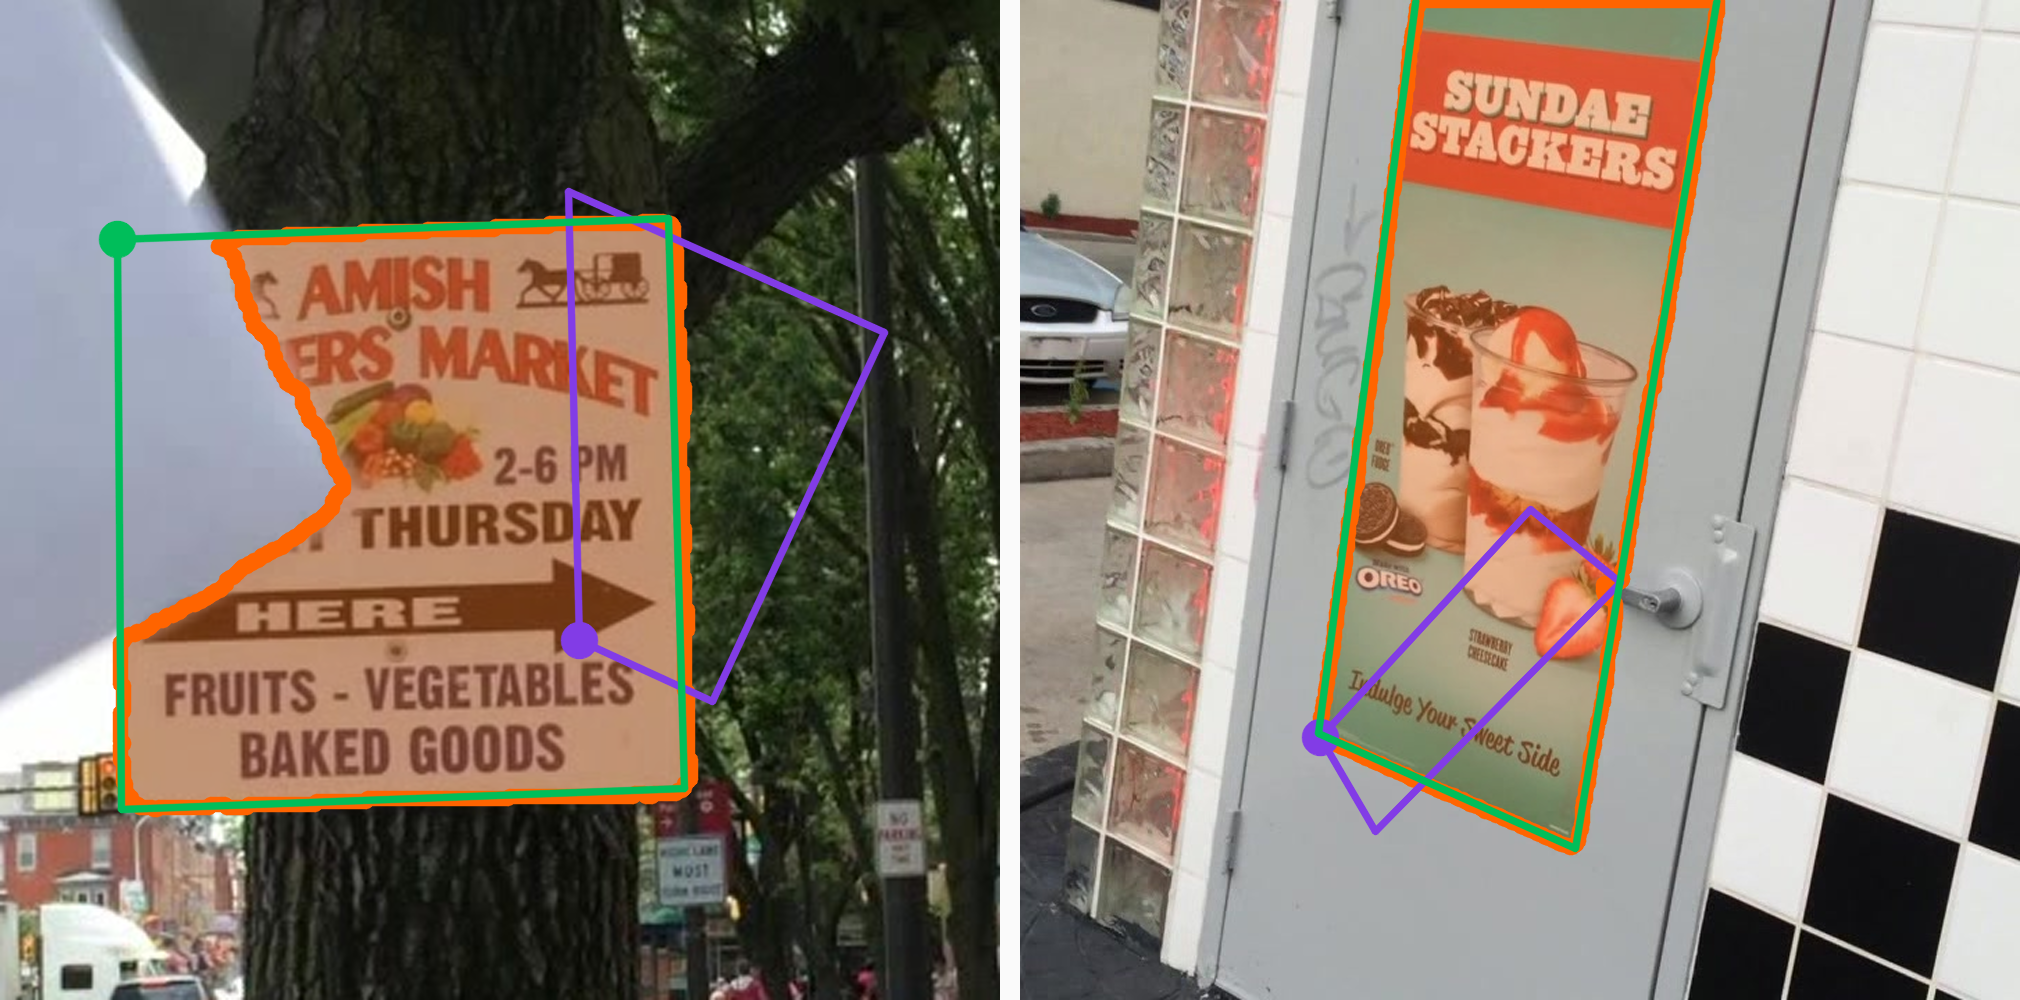
\includegraphics[width=\linewidth]{mask_pose_failure}
    \caption{Correct segmentation, wrong mask-derived pose, on POT-210:
    \texttt{V22\_5} frame 171 (left) and \texttt{V29\_3} frame 251 (right).
    The \textcolor{sam3color}{SAM3 mask} covers the visible target in both frames, yet the \textcolor{maskposecolor}{pose fitted to it} misses the \textcolor{gtcolor}{ground truth} by 184 and 365 pixels, while the keypoint branch is within 0.7 and 1.6 pixels.
    An occluder cuts the silhouette on the left; the target crosses the image border on the right.
    Line extraction is not what fails: three of the four target edges are recovered to under 2 pixels in both frames.}
    \label{fig:mask-pose}
\end{figure}

\Cref{fig:mask-pose} shows the same step failing where neither the mask nor the line fit is at fault.
On both frames the mask covers the target (0.99 IoU against the annotated quadrilateral on the right panel, 0.99 precision on the left) and three of its four edges are recovered within 2 pixels; the fourth is missing, because the occluder and the image border replace one true edge with a truncation edge.
The consequence is structural: the branch converts lines into corner intersections and requires four of them for a direct estimate, so with two or three it falls back to a similarity transform composed onto its own previous pose and the recovered lines are discarded.
Over the two sequences the correlation is exact --- every frame with four surviving intersections estimates directly and overlaps its own mask by 0.98--0.99 IoU, while every frame with two or three drops to 0.00--0.40 in a single step and recovers just as abruptly when the fourth corner returns.
Mask quality therefore cannot predict this failure, and its cost is not proportional to how much of the target is hidden.
It is also why the branch is worth keeping separate rather than fusing: on both frames the keypoint branch is within 1.6 pixels, and the selection rule of \cref{sec:pose-selection} takes it.

\subsection{Efficiency}
\label{sec:efficiency}

On an A100-SXM4, averaged over three 100-frame \pttst sequences after five warm-up frames, the tracker runs at 286.7\,ms per frame (3.49 FPS) with a 6.45\,GB peak measured on a separate 120-frame sequence.
The naming rule is close to free: it adds four homography evaluations and reprojects matches the keypoint branch has already computed, costing 0.1\,ms against no naming at all --- within measurement noise --- and running 4.5\% faster than the DINOv2 appearance vote it replaces (299.5\,ms, 6.53\,GB), which it also removes from memory.
The tracker as a whole is not real-time; SAM3 and \loma dominate that cost, and neither is a contribution of this paper.
% ===== sec/5_limitations =====
\section{Limitations}
\label{sec:limitations}

\flatsam inherits the quadrilateral assumption of \samh: four stable mask-boundary lines are needed for a full mask-derived homography.
Partial visibility reduces this branch to a similarity transform or translation composed onto its previous pose, which discards correctly fitted boundary lines: \cref{fig:mask-pose} shows three edges recovered within 2 pixels and a pose still hundreds of pixels wrong, because the fourth intersection is missing.
Estimating directly from the visible lines, rather than from four corner points, would remove this cliff.

Both branches consume the same SAM3 mask because it defines the keypoint sampling region.
Background keypoints are the intended fallback for a wrong or late mask, but our ablation prices the preference, not the fallback.
Their pose states are independent, but a segmentation failure can remove keypoints and damage both estimates.
UCSB further shows two mask-branch risks: segmentation can target a different physical region from the benchmark annotation, and quadrilateral fitting can fail despite an aligned mask.

Finally, the 35-inlier selection rule leaves 3.1\,pp of oracle headroom on \pttst and 0.9\,pp on POT, and has a per-frame discontinuity.
Its broad sensitivity plateau limits dependence on the exact value, but continuous confidence or calibrated combination remains open.
% ===== sec/5_conclusion =====
\section{Conclusion}
\label{sec:conclusion}

\flatsam estimates a planar pose from correspondences between the initial and the current frame, fitted by MAGSAC, with no pre-warp and no rectification step.
That classical recipe becomes competitive only once the keypoint budget is focused on the target by the tracked segmentation mask: on PlanarTrack it is worth 13.7\,pp of p@15 over the same matcher applied to whole frames.
A mask-derived branch covers what correspondences cannot, and the same raw correspondences name its cyclically equivalent corners, replacing a second appearance network with one bounded support score.
The two branches share a segmentation stream and nothing else, which replaces the prior cascade with one comparison and makes each branch separately measurable --- and they invert between the benchmarks, which is why previous trackers led one of them at a time.
\flatsam leads both, 98.5 p@15 on POT-210 and 88.0 on PlanarTrack, and five of six benchmarks overall; UCSB, where dense flow remains stronger, is analyzed in \cref{sec:failure-analysis}.
% ===== sec/6_acknowledgements =====
\section{Future Work}
\label{sec:future}
We see four research directions.

\begin{itemize}
\item \textbf{Mask-to-homography beyond quadrilaterals.}
This is the major one.
In the general setting --- a fresh re-detection after a tracking failure, an occlusion, or an out-of-view period --- the problem is very hard.
The mask may be partially occluded or inaccurate; the shape may be symmetric, up to infinitely many symmetries for a circle; the objective has many local optima, from the symmetries but not only from them; and aligning boundaries in the space of homographies is difficult, as methods such as iterative closest point that work well for translation and rotation mostly fail for homographies.
The plain $3\times3$ matrix form is numerically poor: its entries live on very different scales, and the perspective terms can easily blow up the whole estimate.
Hierarchical, coarse-to-fine schemes --- fit a translation first, then add rotation, and so on --- did not work well for us either.
The loss must be robust to partial occlusions and small segmentation errors.
A learned approach may do better than classical optimization here.

\item \textbf{Knowing which branch to trust.}
A reliable way to tell whether, or to what extent, the correspondence and the mask branch can be trusted, and what to do when they disagree on the pose.
This need not be a per-frame decision: the target may have no texture in the initial frame, or the keypoint branch may have failed for $N$ consecutive frames, and either could disqualify a branch for a while.
Ideally the decision is ``intelligent''; vision-language models are one candidate, either for the decision itself or for gathering training examples and pseudo-labels.

\item \textbf{Mask correction.}
Once branch quality is known, the pose could correct the SAM mask, connecting the two branches in both directions.
This would help when SAM segments the whole box rather than its front face, spills, or jumps to a distractor.
Our SAM3 version already has a correction API, but we do not know when to correct or how to do it effectively: disable the memory update on some frames, add new conditioning frames with our corrections, and at what frequency.
We do not expect large gains, as SAM usually segments well, but story-wise it would be nice.

\item \textbf{A new planar tracking benchmark.}
To support the generalization to non-quadrilateral targets: a benchmark that need not be large but captures new challenges in the style of VOT --- arbitrary shapes, low texture, changing texture, blur, and the other current failure modes.
Targets should span degrees of symmetry and shape complexity, from a circle to a hand silhouette, including long thin shapes and regions that are not ``an object'' at all, such as an arbitrarily shaped sub-surface of a larger plane --- something SAM2 and SAM3 cannot currently segment.
Maybe even something crazy like wire EDM stuff (\url{https://www.youtube.com/watch?v=f9zyenX2PWk} or \url{https://www.youtube.com/watch?v=ekwk5VsflKI}) --- when the two parts are aligned perfectly, their boundary is invisible, then they separate again (hard case for companions and when to trust them, also pretty much texture-less and overall nicely crazy).

\item \textbf{This but with arbitrary other local features}
  Maybe LoMa is not so important here and a segmentation-mask-densified SIFT (or \dots) would work too.
\end{itemize}

\vspace{5mm}
\noindent\textbf{Acknowledgements.}
This work was supported by the National Recovery Plan project CEDMO 2.0 NPO (MPO 60273/24/21300/21000), the EC Digital Europe Programme project CEDMO 2.0 no.\ 101158609, and by the Research Center for Informatics project CZ.02.1.01/0.0/0.0/16\_019/0000765 funded by OP VVV.

{
    \small
    \bibliographystyle{ieeenat_fullname}
    \bibliography{sjo-bib}
}

\ifcombined\appendix

\section{Additional Method Details}
\label{sec:supp-method}

\noindent\textbf{Mask-derived pose.}
The mask branch reproduces \samh~\cite{serych2026woftsam}; we restate it here so the branch our contribution names corners for is self-contained.
Contours of the binary mask $S_t$ are extracted and fragments shorter than 20 points are discarded.
Contour points adjacent to the image border are marked, because a silhouette edge that coincides with the frame boundary is an artefact of the field of view rather than an object edge.
Tangents are estimated by finite differences with a four-point step and vote into a $(\text{distance},\text{angle})$ accumulator; the four strongest peaks give the dominant boundary lines.
Each line is refit by least squares to the contour points that voted for it, and lines with no support or a supported segment shorter than five pixels are dropped.
Intersections of the remaining line pairs are corner candidates, kept only within 80 pixels of a contour point.

\noindent\textbf{Correspondence and partial visibility.}
Candidate corners carry no identity, so all injective assignments between the four template corners and the surviving intersections are enumerated.
Two-corner assignments are required to be consistent: a pair of adjacent template corners must map to intersections that share a line, and a pair of opposite corners must not.
Only the surviving assignments of maximal size are scored.
Every assignment yields a transformation whose form depends on how many corners it uses: four or more give a full homography by DLT, two or three give a similarity composed onto the branch's previous homography, one gives a translation, and none leaves the previous homography unchanged.
The scored quantity is displacement from the branch's own previous prediction, so the accepted candidate is the one closest to the incumbent pose --- a zero-motion prior, not a fit quality.
Because two and three corner cases are resolved against the previous pose, the branch is a frame-to-frame composition exactly while the target is partly visible, and returns to an initial-to-current estimate as soon as four corners are recovered.

This is also where the cyclic ambiguity enters.
Selecting the candidate nearest the incumbent propagates the incumbent's labelling instead of testing it: when the incumbent is mis-named, the assignment closest to it is the equally mis-named one, and a similarity or translation update inherits that labelling unchanged.
A mis-naming therefore persists until evidence from outside the mask breaks the tie.
\Cref{sec:match-naming} is that tie-breaker.

\section{Naming Sensitivity}
\label{sec:supp-naming}

We sweep naming parameters on 50 PlanarTrack training sequences rather than selecting them on the reported test split.
The sweep scores whether each parameter setting selects the cyclic naming that ground truth prefers for the mask-branch pose; it is a decision-level analysis, not an end-to-end p@15 re-run.

\begin{table*}[t]
    \centering
    \setlength{\tabcolsep}{4pt}
    \begin{tabular}{lrrrrrrrrr}
        \toprule
        $\tau$ (px) & 3 & 5 & 7 & 10 & 15 & 20 & \textbf{30} & 50 & 100\\
        \midrule
        naming accuracy & 99.35 & 99.37 & 99.36 & 99.38 & 99.38 & 99.37 & 99.37 & 99.37 & 99.34\\
        \bottomrule
    \end{tabular}
    \caption{Train-split naming-decision accuracy (\%), holding the raw-match minimum at eight.
    Bold marks the deployed value.}
    \label{tab:supp-tau}
\end{table*}

\begin{table}[t]
    \centering
    \setlength{\tabcolsep}{4pt}
    \begin{tabular}{lrrrrrr}
        \toprule
        minimum matches & 0 & 4 & \textbf{8} & 12 & 16 & 32\\
        \midrule
        naming accuracy & 99.28 & 99.36 & 99.37 & 99.38 & 99.38 & 99.37\\
        \bottomrule
    \end{tabular}
    \caption{Train-split naming-decision accuracy (\%), holding $\tau=30$ pixels.
    Bold marks the deployed value.}
    \label{tab:supp-min-matches}
\end{table}

Accuracy in \cref{tab:supp-tau,tab:supp-min-matches} varies by only 0.04\,pp over the full $\tau\in[3,100]$ range and by 0.10\,pp for raw-match minima from zero to 32.
The claim is the flatness, not the maximum: accuracy peaks at $\tau=10$--$15$ and the deployed $\tau=30$ is 0.01\,pp below it, so adopting the argmax would be tuning on the sweep rather than choosing inside a plateau.
One coverage caveat applies to \cref{tab:supp-min-matches}: every localized frame of this train sample carries at least eight raw matches, against 87.2\% of frames on \pttst, where the remaining 12.8\% abstain and keep the incumbent naming.
The minimum-match plateau therefore describes the rule's accuracy where it fires, not the cost of the abstentions it causes in deployment.

\section{Additional Results}
\label{sec:supp-results}

\Cref{tab:supp-cross-full} gives the cross-dataset comparison of \cref{tab:cross-dataset} at both precision thresholds and with the corner-naming gap, on all six benchmarks.
Three things are visible that the main table cannot show.
First, the margins over \woftsam are robustness margins rather than precision ones: the lead grows from 8.2\,pp at p@5 to 10.4\,pp at p@15 on \pttst and from 4.4 to 5.6\,pp on TMT, while the saturated POT column narrows from 1.5 to 1.0\,pp.
UCSB is the exception in both directions: the two trackers are within 1.2\,pp at p@5 there, and the deficit opens to 4.4\,pp at p@15, which is the signature of lost frames rather than imprecise ones.
Second, the deployed naming gap is at most 0.03\,pp outside \pttst and exactly zero on two benchmarks, which is what a naming mechanism should look like once it works.
Third, \samh --- the mask branch run alone --- is 29 to 66\,pp behind \woftsam at p@5 on the classical datasets while losing far less at p@15, so its errors are dominated by imprecise poses rather than lost targets; \cref{sec:failure-analysis} shows what one looks like.

\begin{table*}[t]
    \centering
    \setlength{\tabcolsep}{4pt}
    \begin{tabular}{llrrrrrr|r}
        \toprule
        % woftsam_samfallback_nl, sam_H, loma_samh_decoupled_rerun,
        % loma_samh_matchnaming; experiments/results_tables.py.
        method & metric & \pttst & POT-210 & POIC & TMT & UCSB & MPOT-3K & worst\\
        \midrule
        \multirow{3}{*}{\woftsam~\cite{serych2026woftsam}}
        & p@5 & 57.4 & 91.9 & 97.6 & 79.9 & \frst{56.5} & 67.4 & \frst{56.5}\\
        & p@15 & 77.6 & 97.5 & 99.2 & 89.1 & \frst{96.6} & 90.8 & 77.6\\
        & \brgap & 1.55 & \frst{0.00} & \frst{0.00} & 0.63 & \frst{0.03} & 0.30 & 1.55\\
        \midrule
        \multirow{3}{*}{\samh~\cite{serych2026woftsam}}
        & p@5 & 62.4 & 68.6 & 68.4 & 14.3 & 20.9 & 54.7 & 14.3\\
        & p@15 & 80.5 & 89.4 & 80.8 & 54.3 & 54.3 & 82.0 & 54.3\\
        & \brgap & 2.56 & 1.10 & \frst{0.00} & 2.74 & 0.38 & 1.44 & 2.74\\
        \midrule
        \multirow{3}{*}{\flatsam, DINOv2 naming}
        & p@5 & \frst{65.6} & \frst{93.6} & \frst{97.7} & \frst{84.3} & 55.2 & \frst{69.1} & 55.2\\
        & p@15 & 87.7 & \frst{98.5} & \frst{99.3} & 94.5 & 92.2 & \frst{92.6} & 87.7\\
        & \brgap & 1.57 & \frst{0.00} & \frst{0.00} & 0.36 & \frst{0.03} & 0.03 & 1.57\\
        \midrule
        \multirow{3}{*}{\textbf{\flatsam, match naming}}
        & p@5 & \frst{65.6} & 93.4 & \frst{97.7} & \frst{84.3} & 55.3 & 69.0 & 55.3\\
        & p@15 & \frst{88.0} & \frst{98.5} & \frst{99.3} & \frst{94.7} & 92.2 & \frst{92.6} & \frst{88.0}\\
        & \brgap & \frst{1.36} & \frst{0.00} & 0.02 & \frst{0.03} & \frst{0.03} & \frst{0.00} & \frst{1.36}\\
        \bottomrule
    \end{tabular}
    \caption{Complete cross-dataset results: p@5, p@15 and the corner-naming gap $\brgap$ on all six benchmarks.
    Best value per row group in bold; lower is better for $\brgap$.
    The worst column is each method's weakest benchmark for that metric.}
    \label{tab:supp-cross-full}
\end{table*}

\noindent\textbf{MPOT-3K protocol.}
Each annotated planar instance is initialized and tracked as an independent single-target task, giving 573 tasks scored with the same alignment-error precision as every other dataset here.
That isolates per-plane pose accuracy, which is what this paper changes, but it neither detects instances nor maintains identities across them, so it is not comparable to the benchmark's MOTA, IDF1, and success-rate protocol.
\fi

\end{document}
